%% Repairing derived facts in stale KV caches after document edits.
%% IEEE conference template (IEEEtran). Every number comes from the run artefacts in ../results-gpu
%% (out/results.json, out/results_<model>.jsonl, followup/results_followup.json); tables are generated by
%% make_tables.py into tables/.
\documentclass[conference]{IEEEtran}
\IEEEoverridecommandlockouts

\usepackage{cite}
\usepackage{amsmath,amssymb}
\usepackage{graphicx}
\usepackage{textcomp}
\usepackage{xcolor}
\usepackage{booktabs}
\usepackage{multirow}
\usepackage{url}
\usepackage{pgfplots}
\pgfplotsset{compat=1.18}
\usepgfplotslibrary{groupplots}

\definecolor{seriesA}{HTML}{2A78D6}
\definecolor{seriesB}{HTML}{EB6834}
\definecolor{seriesC}{HTML}{1BAF7A}
\definecolor{gridline}{HTML}{E4E3DF}
\newcommand{\ci}[2]{{\scriptsize[#1,\,#2]}}
\makeatletter\newcommand{\tablebody}[1]{\@@input #1 }\makeatother

\begin{document}

\title{How Far Does an Edit Reach?\\
{\Large Repairing Derived Facts in Stale KV Caches}}

\author{\IEEEauthorblockN{Nour Shreif, Hadi Ghazi, Karin Zoabi}
\IEEEauthorblockA{\textit{Lebanese University}}}

\maketitle

\begin{abstract}
When a cached document is edited, the cached states of text that depends on the edit become stale, and
repairing them means recomputing part of the cache. The published policies recompute a fixed window after
the edit or a window at the text that carries the answer; both fail when the answer is a derived fact stated
far from the edit, and the contiguous window from the edit to the dependent text has been proposed but not
tested. We build a benchmark of derived-fact edits on Qwen3-8B, Llama-3.1-8B and Mistral-7B, varying the
distance to the dependent text (0 to about 1,700 tokens), the number of hops (2 or 3) and the number of
dependent facts (1 or 3), with checks that the full re-read answers correctly and the stale cache does not. A
path window whose stopping point comes from a word index built at edit time recovers the answer margin almost
completely in every explicit-dependency cell on all three models (margin recovery 0.99 to 1.00, answer accuracy 95
to 100\%) while
recomputing 29 to 65\% of the tokens that recomputing to the end needs. A fixed window at the same average
cost recovers 0.44 to 0.81, the carrier window fails on Llama, falls short on Mistral and fails on every model at
three hops, an
appended erratum works on Llama but answers correctly only 11 to 54\% of the time on the other two, and a
dependency graph built by a small LLM before the edit recovers 0.09 to 0.53. Controls show that what repairs
the cache is reaching the dependent sentences together with the text that carries the edit to them: random
positions at the same budget recover at most 0.36, and the gap without the dependent sentences recovers
nothing. When the dependency is paraphrased (``the sixth plan'' against ``Plan six''), the path window still
repairs the cache if it knows where to stop, but the word index cannot find the dependents; a gpt-4.1
dependency graph built before the edit, combined with one asked at edit time, recovers 0.84 to 0.98. A graph
asked only at edit time finds the text the edit made relevant and misses the text it made irrelevant, whose
stale states still assert the old answer (0.21 against 1.01, depending on which comes first). Positions picked
by attention to the edited sentence also succeed at a fixed 512 tokens in every cell, including paraphrased
ones, but they need the model's attention statistics and a budget that is not known in advance.
\end{abstract}

\begin{IEEEkeywords}
KV cache, document editing, cache repair, retrieval-augmented generation, ripple effects
\end{IEEEkeywords}

%% ------------------------------------------------------------------------------------------------
\section{Introduction}

Serving systems keep the key-value (KV) cache of long documents so that later questions do not pay for
re-reading them. When a document is edited, every cached state computed after the edited text was computed
from the old version, and the cache is stale. Re-reading the whole document restores it but costs a full
prefill, so a repair policy recomputes only part of the cache. Mao et al.~\cite{mao2026contiguity} compare such
policies at a fixed budget and find that a contiguous window recomputed right after the edit (EditLocal) beats
importance-based selection, but that it fails when the answer is a derived fact stated far from the edit: an
edited alias that selects between two unchanged lookup rows 250 or 1,500 tokens later. A window placed at
those rows (CarrierWindow, which needs an oracle) works on Qwen and much less on Llama. The authors name a
window spanning the path from the edit to the dependent text as the natural next step and leave it untested.
A different line appends a correction instead of recomputing~\cite{li2026programmable}, tested on direct
policy facts but not on derived ones at a distance.

We test the path window, and we ask what any policy has to recompute for a derived fact to be repaired. The
practical obstacle is knowing where the dependent text ends. We find it with a deployable rule built at edit
time: a word index that starts from the words the edit changed and follows the rare names and codes of the
sentences it reaches. For dependencies that share no word with the edit we follow our earlier proof of concept,
which combined such an index with an LLM-built dependency graph, and test LLM graphs built before the edit and
queried at edit time. Our contributions are:
\begin{itemize}
\item a benchmark of derived-fact edits that varies distance, hops, fan-out, distracting mentions of the
edited entity and paraphrased dependencies, with every edit length-preserving in three tokenizers and
per-model checks that the full re-read answers correctly and the stale cache does not (Section~\ref{sec:bench});
\item a comparison of 40 repair policies on Qwen3-8B, Llama-3.1-8B and Mistral-7B, in which the edit-time path
window is the only model-free policy that repairs every explicit-dependency cell on every model at less than
the cost of recomputing to the end (Section~\ref{sec:results});
\item controls that locate what repair requires: the dependent sentences and the text that carries the edit to
them, rather than a budget large enough (Section~\ref{sec:controls});
\item for paraphrased dependencies, evidence that a strong LLM can find the dependents, that a complete
dependency set must include the text the edit made irrelevant as well as the text it made relevant, and that
combining a graph built before the edit with one queried at edit time covers both (Section~\ref{sec:indirect});
\item evidence that the erratum is strongly model-dependent, and that positions picked by stored attention, as
in PatchKV, can repair at long range if their budget is large enough, while they fail at the 32-token budget
Mao et al.\ tested (Sections~\ref{sec:results} and~\ref{sec:controls}).
\end{itemize}

%% ------------------------------------------------------------------------------------------------
\section{Related Work}

\textbf{Repairing stale caches.} Mao et al.~\cite{mao2026contiguity} define the in-place repair problem, the
margin-recovery metric we use, the derived alias-to-lookup benchmark we extend, and the EditLocal and
CarrierWindow policies; their code is not released, so we reimplement both. PatchKV~\cite{yang2026patchkv}
repairs dynamically edited contexts with an edit-local window plus distant blocks chosen by stored attention, on
multi-hop QA workloads without a derived-fact construction. Chunk-reuse methods such as
CacheBlend~\cite{yao2025cacheblend} recompute selected tokens when independently cached chunks are joined, a
related but different staleness. Li~\cite{li2026programmable} argues that the cache stores the model's notes
about the text, and that appending an erratum is a cheap, robust way to change a decision; its tests use gated
policy facts on one model, and its two-hop refreshes of the edited field alone recover almost nothing. Cai and
Cai~\cite{cai2026eventkv} discuss when appended corrections are preferable to edits in sparse event caches.

\textbf{Ripple effects.} Knowledge-editing work calls the downstream consequences of an edited fact its ripple
effects~\cite{cohen2024ripple} and tests them with multi-hop questions~\cite{zhong2023mquake}. Our cells play
the same role for a cached document instead of model weights.

%% ------------------------------------------------------------------------------------------------
\section{Benchmark}
\label{sec:bench}

\textbf{Items.} Each document is real WikiText-103 text~\cite{merity2017wikitext} (validation paragraphs with
none of the benchmark's names or code-like tokens) with a few inserted sentences. About 600 tokens of text
precede the edited sentence, so recomputing to the end is cheaper than a full re-read, and about 600 tokens
follow the last dependent sentence. Nine cells of 50 items each:
\begin{itemize}
\item \emph{direct}: the edited sentence states the code itself (``Company Varnex's code is Q7'' becomes
``R6''), a check that refreshing the edit is enough;
\item \emph{derived}, $d \in \{0, 250, 1500\}$: Mao et al.'s construction. ``Company Varnex uses alias Delta''
becomes ``Lambda'', and two unchanged rows (``Alias Delta maps to code Q7'', ``Alias Lambda maps to code R6'')
follow at distance $d$, in random order;
\item \emph{3 hops}: alias rows map to groups and group rows map to codes, each pair about 250 tokens further;
\item \emph{fan-out 3}: three attribute pairs (code, tag, room) about 250 tokens apart; the question asks for one;
\item \emph{noisy}: the derived cell at $d=250$ with four extra sentences about the same company (office, staff,
founding year, sponsorship) in the gap and the tail;
\item \emph{indirect}, $d \in \{250, 1500\}$: the derived construction with no shared word, taken from our proof
of concept. ``Company Varnex uses the third plan'' becomes ``the sixth plan'', and the rows read ``Plan three
maps to code Q7'' and ``Plan six maps to code R6'', in random order.
\end{itemize}
The question gives the rule (``Company Varnex's code is the code of the alias it uses'') and asks for the code.
Measured distances from the end of the edit to the first dependent sentence have medians of 317 to 362 tokens
in the $d=250$ cells and 1,500 to 1,740 in the $d=1500$ cell; documents run from about 1,450 to 3,550 tokens.

\textbf{Validity.} Every edit changes a contiguous run of tokens inside the edited sentence and leaves the
token count unchanged in all three tokenizers, so cached positions stay aligned; items that fail this in any
tokenizer are redrawn. Each model then keeps an item only if the full re-read improves the new-minus-old
margin over the stale cache by at least one nat per token and prefers the new answer, the full re-read
generates the new code, and the stale cache does not. Qwen3 keeps 322 of the 350 explicit-dependency items,
Llama 263 and Mistral 260. The rejects are items with too small a margin gain (12, 40 and 26 for Qwen3, Llama and
Mistral), items whose full re-read did not generate the new code (12, 21 and 42), and items whose stale cache
already generated it (4, 26 and 22). The indirect items are harder: even
after a full re-read, the models often cannot resolve ``the sixth plan'' to ``Plan six'', and they keep 61, 25
and 32 of 100.

%% ------------------------------------------------------------------------------------------------
\section{Policies and Setup}

\textbf{Policies.} Every policy starts from the stale cache and recomputes a set of positions of the edited
document with the same operator; we report the tokens it recomputes.
\begin{itemize}
\item \emph{Floors and ceilings}: no repair; the edited tokens only; recompute from the edit to the end
(\emph{suffix}); a full re-read (\emph{full}).
\item \emph{Fixed windows}: EditLocal with $K \in \{32, 64, 128, 256, 512, 1024\}$ tokens after the edit, and a
window to the end of the edited paragraph.
\item \emph{Oracle carriers}: Mao's CarrierWindow (32 tokens from the first row the question needs), and the
dependent sentences alone (\emph{rows}).
\item \emph{Path windows}: recompute from the edit to the end of the furthest dependent sentence, found by the
construction's ground truth (oracle), by the \emph{edit-time index}, by an LLM graph, or by both.
\item \emph{Erratum}~\cite{li2026programmable}: append ``[STATE UPDATE] Company Varnex: alias $\rightarrow$
Lambda (was Delta). This overrides any earlier value and conclusion.'' after the document, with the cache left
stale, with the edited tokens refreshed, or with EditLocal@32.
\item \emph{Attention}: rank downstream positions by the attention they paid to the edited sentence during the
original prefill (every fourth layer, averaged over heads), and recompute the top positions or 32-token
blocks, at the path window's budget or at a fixed 32, 128 or 512; or stop where that attention falls below 25\%
or 10\% of its maximum.
\item \emph{Controls}: random positions or random 32-token blocks at the path window's budget, and the gap from
the edit up to the first dependent sentence without that sentence (\emph{StopShort}).
\end{itemize}

\textbf{Edit-time index.} The index needs no model. It takes the words that differ between the old and new
edited sentence (here the two aliases), marks every later sentence containing one of them, then adds the
names and codes (capitalised words or words containing a digit) that occur in at most three sentences of the
document and follows them for up to three hops. The path window recomputes up to the end of the furthest
sentence reached. The \emph{LLM graph} instead asks gpt-4o-mini, once per document and before any edit, for
the sentence-level dependency edges of the original text, and follows them from the edited sentence; it cost
US\$0.18 for all 350 explicit-dependency documents. On the indirect cells we build this graph with gpt-4o-mini
and with gpt-4.1, and we also ask each model \emph{at edit time}, given the old and new edited sentence, which
later sentences depend on it; the path window then stops at the furthest sentence any chosen source reaches.
These graphs cost US\$1.55 for the 100 indirect documents.

\textbf{Models and runtime.} Qwen3-8B~\cite{qwen2025qwen3}, Llama-3.1-8B-Instruct~\cite{dubey2024llama3} (the
ungated mirror of the same weights) and Mistral-7B-Instruct-v0.3~\cite{jiang2023mistral}, in bfloat16 on one
L40S GPU each. The document sits in the user turn of each model's chat template, with the question after it.
Repair uses our own forward pass over a preallocated cache, so that any set of positions can be recomputed in
place, each attending to every cached key at or before it. Before each run it is checked against the library:
the last-token logits differ by at most 0.8\% of their range with identical top-5 tokens, and recomputing
every position of a stale cache reproduces a fresh prefill exactly.

\textbf{Metrics.} Margin recovery (MR)~\cite{mao2026contiguity} is $(m - m_\text{stale}) / (m_\text{full} -
m_\text{stale})$, where $m$ is the length-averaged log-probability of the new answer minus that of the old
one: 0 is no better than the stale cache and 1 is as good as a full re-read. Accuracy is the share of items
whose greedy answer (up to 8 tokens) contains the new code and not the old. We report means with item-level
bootstrap 95\% intervals~\cite{efron1993bootstrap}. A second run of seven reference policies on a fresh pod
reproduced every item's MR exactly.

%% ------------------------------------------------------------------------------------------------
\section{Results}
\label{sec:results}

\begin{table*}[t]
\centering
\caption{Margin recovery (mean; 1 = as good as a full re-read) on the derived cells. Bold: the path window
with the edit-time index. el32: EditLocal@32; carrier: Mao's CarrierWindow (oracle); rows: the dependent
sentences only (oracle); erratum: edited tokens plus appended correction; LLM graph: path window from a
graph built before the edit; random: random positions at the path window's budget; StopShort: the gap without
the dependent sentences; attn: positions ranked by attention to the edited sentence, fixed budget.}
\label{tab:mr}
\footnotesize
\setlength{\tabcolsep}{3.6pt}
\begin{tabular}{llcccccccccc}
\toprule
Model & Cell & el32 & carrier & rows & erratum & LLM graph & random & StopShort & attn@128 & attn@512 & path (index) \\
\midrule
\tablebody{tables/t_mr.tex}
\bottomrule
\end{tabular}
\end{table*}

\begin{table*}[t]
\centering
\caption{Answer accuracy (\%, greedy answer contains the new code and not the old) for the same policies and
cells as Table~\ref{tab:mr}.}
\label{tab:acc}
\footnotesize
\setlength{\tabcolsep}{3.6pt}
\begin{tabular}{llcccccccccc}
\toprule
Model & Cell & el32 & carrier & rows & erratum & LLM graph & random & StopShort & attn@128 & attn@512 & path (index) \\
\midrule
\tablebody{tables/t_acc.tex}
\bottomrule
\end{tabular}
\end{table*}

\begin{table*}[t]
\centering
\caption{Indirect cells (``the sixth plan'' against ``Plan six''): margin recovery of the path window by how the
dependents are found, against attention@512 and the oracle. $n$: items kept. Before: graph built from the
original document; at edit: the model asked, given the old and new edited sentence, which later sentences
depend on it; both: the path window stops at the furthest sentence either reaches. Accuracy is for ``both''.}
\label{tab:indirect}
\footnotesize
\setlength{\tabcolsep}{4pt}
\begin{tabular}{llccccccccc}
\toprule
Model & Cell & $n$ & word index & gpt-4o-mini before & gpt-4.1 before & gpt-4.1 at edit & gpt-4.1 both & attn@512 & oracle & acc.\ (\%) \\
\midrule
\tablebody{tables/t_indirect.tex}
\bottomrule
\end{tabular}
\end{table*}

\textbf{The path window repairs every explicit-dependency cell.} With the edit-time index, the path window reaches MR 0.99 to 1.00
and 95 to 100\% accuracy in all eighteen derived cells (Tables~\ref{tab:mr} and~\ref{tab:acc}). The index
found every dependent sentence and no other sentence on every item, so the oracle path window gives identical
numbers. On the direct cell, where the index stops at the edit itself, refreshing the two edited tokens already
recovers 0.91 to 0.96.

\textbf{Fixed windows cannot know how far to go.} EditLocal@32 repairs the adjacent rows ($d=0$, MR 1.00) and
nothing beyond them (MR at most 0.06 in every other derived cell), which reproduces Mao et al.'s 0.01 to 0.09
at $d=250$. Larger fixed windows do not close the gap at equal cost (Fig.~\ref{fig:frontier}): a fixed window
spends its budget on near items and falls short of far ones, so at the path window's mean cost a fixed window
recovers 0.44 to 0.81 (log-interpolated between the two neighbouring budgets of the EditLocal sweep, where that
cost lies inside the sweep), and even 1,024 tokens recover nothing at $d=1500$.

\begin{figure}[t]
\centering
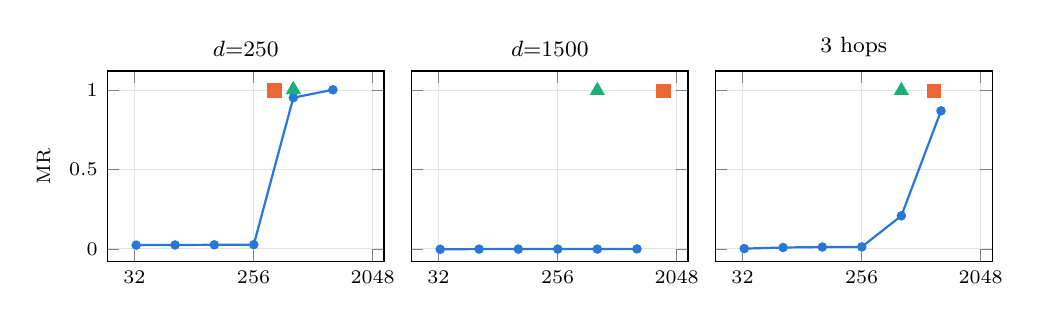
\begin{tikzpicture}
\begin{groupplot}[group style={group size=3 by 1, horizontal sep=0.35cm, y descriptions at=edge left},
  width=0.42\columnwidth, height=4.0cm, xmode=log, xmin=20, xmax=2500, ymin=-0.08, ymax=1.12,
  xtick={32,256,2048}, xticklabels={32,256,2048}, xticklabel style={font=\scriptsize}, yticklabel style={font=\scriptsize},
  grid=major, grid style={gridline}, title style={font=\footnotesize, yshift=-1ex}]
\nextgroupplot[title={$d{=}250$}, ylabel={\scriptsize MR}, legend to name=frontierlegend, legend columns=3, legend style={font=\scriptsize, draw=none}]
\addplot[seriesA, thick, mark=*, mark size=1.3pt] coordinates {(33,0.023) (65,0.024) (129,0.025) (257,0.026) (513,0.952) (1024,1.002)};
\addplot[seriesB, only marks, mark=square*, mark size=2.4pt] coordinates {(368,0.998)};
\addplot[seriesC, only marks, mark=triangle*, mark size=2.8pt] coordinates {(513,1.003)};
\legend{EditLocal (fixed $K$), path window (index), attention@512}
\nextgroupplot[title={$d{=}1500$}]
\addplot[seriesA, thick, mark=*, mark size=1.3pt] coordinates {(33,-0.003) (65,-0.002) (129,-0.002) (257,-0.002) (513,-0.002) (1025,-0.001)};
\addplot[seriesB, only marks, mark=square*, mark size=2.4pt] coordinates {(1628,0.995)};
\addplot[seriesC, only marks, mark=triangle*, mark size=2.8pt] coordinates {(513,0.997)};
\nextgroupplot[title={3 hops}]
\addplot[seriesA, thick, mark=*, mark size=1.3pt] coordinates {(33,0.001) (65,0.008) (129,0.011) (257,0.012) (513,0.208) (1025,0.869)};
\addplot[seriesB, only marks, mark=square*, mark size=2.4pt] coordinates {(905,0.996)};
\addplot[seriesC, only marks, mark=triangle*, mark size=2.8pt] coordinates {(513,0.997)};
\end{groupplot}
\end{tikzpicture}

\ref{frontierlegend}
\caption{Margin recovery against tokens recomputed (log scale), mean over the three models. A fixed window
recovers only once $K$ passes the dependent text, which differs per item; the path window stops at the right
place on each item.}
\label{fig:frontier}
\end{figure}

\begin{table}[t]
\centering
\caption{Mean tokens recomputed (mean over models): the path window, recompute to the end, and a full
re-read, with the path window's share of the full re-read.}
\label{tab:cost}
\footnotesize
\begin{tabular}{lcccc}
\toprule
Cell & path & suffix & full & path/full \\
\midrule
\tablebody{tables/t_cost.tex}
\bottomrule
\end{tabular}
\end{table}

\textbf{It costs a fraction of the alternatives that also work.} Recomputing to the end also recovers 1.00,
and so does a full re-read; the path window recomputes 29 to 65\% of the suffix's tokens and 18 to 50\% of
the full re-read's in the distant cells (Table~\ref{tab:cost}). The saving is the text after the last
dependent sentence, so it shrinks when dependents sit near the end of the document.

\textbf{The carrier window depends on the model and fails at three hops.} Recomputing 32 tokens at the rows
the question needs recovers 0.92 to 0.95 on Qwen3 at every distance but 0.30 to 0.46 on Llama and 0.56 to 0.69
on Mistral, as Mao et al.\ found for Qwen and Llama. With three hops it recovers nothing on any model; the row the question needs is the second stage, and the
group rows it builds on stay stale.

\textbf{The erratum is cheap but unreliable.} Appending a 26 to 34-token correction to a cache whose edited
tokens are refreshed gives 68 to 100\% accuracy on Llama, but 29 to 54\% on Qwen3 and 11 to 43\% on Mistral,
and it is weakest at three hops and fan-out. MR exceeds 1 on Llama because the erratum adds evidence a re-read
of the edited document does not contain.

\textbf{A graph built before the edit misses dependencies.} The LLM graph recovers 0.84 to 0.85 when the rows
are adjacent but only 0.09 to 0.53 elsewhere. Its edges reach 76\% of the dependent sentences when they are
adjacent, 53\% at $d=250$, 27\% at $d=1500$, 25\% at three hops, 15\% at fan-out and 9\% in the noisy cell. It
also favours the rows of the old alias, which the original document's logic uses, over those of the new alias,
which the edit makes relevant (48\% against 24\% at three hops). The edit-time index reaches every dependent
sentence because it starts from the words the edit changed.

%% ------------------------------------------------------------------------------------------------
\section{Paraphrased Dependencies}
\label{sec:indirect}


\begin{table}[t]
\centering
\caption{Indirect cells pooled over models and distances, split by which of the two rows comes first: margin
recovery of the gpt-4.1 path windows (61 item-model pairs with the new plan's row first, 57 with the old plan's).}
\label{tab:order}
\footnotesize
\begin{tabular}{lcc}
\toprule
Dependents found by & new row first & old row first \\
\midrule
\tablebody{tables/t_order.tex}
\bottomrule
\end{tabular}
\end{table}

\textbf{The repair still works; finding the dependents is the problem.} When the stopping point is known, the
path window recovers 0.98 to 1.02 on the indirect cells as well (Table~\ref{tab:indirect}). The word index finds
no dependent sentence (its recall is 0.00 to 0.02), so it stops early or at a filler sentence that happens to
contain ``third'' or ``sixth'', and recovers 0.11 to 0.42. gpt-4o-mini fails as well, before the edit (recall 0.02
to 0.09) and at edit time (0.00 to 0.02). gpt-4.1 finds most dependents: its graph built before the edit reaches
66 to 75\% of them and recovers 0.73 to 0.94, and asked at edit time it reaches 54 to 57\% and recovers 0.38 to
0.77. Combining the two recovers 0.84 to 0.98, with 80 to 97\% correct answers. Attention@512 recovers 0.98 to
1.03 here too, without any graph.

\textbf{A dependency set must include what the edit made irrelevant.} The edit-time query is reliable when the
old plan's row comes first and fails when the new plan's row comes first (Table~\ref{tab:order}: 1.01 against
0.21). Asked about the edited sentence, the model returns the row the edit made relevant and leaves out the row
of the old plan. When that row comes later, the path window stops before it, and its stale states, computed
while the old plan was in force, still treat its code as the company's code. A graph built before the edit
links the edited sentence to the old plan's row, so the two sources see complementary halves, and their
combination is close to the oracle whichever row comes first (0.86 and 1.01). The swapped documents of our proof
of concept showed the mirror image for explicit dependencies: a graph built before the edit misses the row
the edit makes relevant.

%% ------------------------------------------------------------------------------------------------
\section{What Repair Requires}
\label{sec:controls}

\textbf{Location, not budget.} Spending the path window's exact budget on random positions recovers 0.00 to
0.36, and on random 32-token blocks at most 0.56. The budget alone does not repair the cache.

\textbf{The dependent sentences are necessary.} StopShort, which recomputes the whole gap but stops before the
first dependent sentence, recovers at most 0.05 in every distant cell on every model.

\textbf{On two models they are not sufficient.} Recomputing the dependent sentences alone recovers 0.85 to
0.94 on Qwen3 but 0.27 to 0.46 on Llama and 0.56 to 0.69 on Mistral. On those models the text between the edit
and the rows also carries the old alias forward, and repairing it is part of the repair. This is the mechanism
behind the carrier window's model dependence.

\textbf{Attention can find the places, not the budget.} Positions ranked by the attention they paid to the
edited sentence recover 0.99 to 1.00 at the path window's budget in every distant cell, and 0.98 to 1.00 at
a fixed 512 tokens, which is
cheaper than the path window when the dependents are far (512 against about 1,600 tokens at $d=1500$ and
fan-out 3). At 32 tokens they recover at most 0.15 at a distance and at 128 tokens 0.35 to 0.96, so the
budget they need is not known in advance; the two stopping rules we fixed before running were unreliable
(25\%: at most 0.14 at a distance; 10\%: $-0.03$ to 1.00). Attention needs no notion of shared words, and at 512 tokens it
also repairs the paraphrased cells (0.98 to 1.03). It does need the attention that downstream positions paid to
the edited span, which a deployed system would have to store at prefill time or pay for at edit time; we did not
charge that cost. These results agree with both earlier papers rather than contradicting Mao et al.'s
``contiguity, not importance'': at their 32-token budget, attention-ranked positions fail here too, and the
success at 512 tokens matches PatchKV's use of stored attention to choose distant blocks~\cite{yang2026patchkv}.

%% ------------------------------------------------------------------------------------------------
\section{Discussion}

A derived fact is repaired when the recomputed set contains the sentences that use the edited value and, on
some models, the text that carries it to them. A fixed budget cannot guarantee that, because how far an edit
reaches is a property of the document. For explicit dependencies, the edit-time index answers that question
without touching the model: it costs one pass over the document's words, needs no prefill statistics and no LLM
call at edit time, and gives each item its own stopping point. For paraphrased dependencies it fails, and a
strong LLM is needed; a small one is not enough on documents of this length. Attention selection is the strongest model-internal alternative and
the cheaper one at long range, provided its statistics are available and its budget happens to be large
enough; combining the index's stopping point with attention-ranked positions inside it is a natural next
policy. A dependency set has two halves: the text the edit makes relevant and the text it makes irrelevant,
whose stale states still assert the old conclusion. A graph of the original text sees the second half and
cannot contain links the edit creates; a question asked at edit time about the new sentence sees the first
half and misses the second. Any practical builder therefore has to look at both versions of the edited
sentence, as the word index does by construction and as the combination of the two LLM graphs does. The
edit-time LLM query has a price the word index does not: an API call takes seconds, while in our runtime the
path window's repair takes about 50 ms and a full re-read about 200 to 225 ms (medians). It is practical as a
background step or as a fallback when the word index finds no dependent sentence, not on the critical path of
every edit. Finally, the erratum's success on one model and failure on two others suggests that
whether a model trusts a late correction over earlier text is a model property, which a policy cannot assume.

\section{Limitations}

Most dependencies are explicit: in seven of nine cells every dependent sentence repeats the alias or group name,
which suits a word index. Its perfect precision on those cells is built in: the background text was filtered so
that no benchmark name or code appears in it, so the index could not make a false hit; on the indirect cells,
whose filler was not filtered for ordinals, it reached 2.1 and 3.8 unrelated sentences per document on average at the two distances. Every
dependency is an inserted template sentence in real background text; we test no real documents or real
edits. The paraphrased cells cover one kind of rewording, and the models keep few of their
items (25 and 32 of 100 for Llama and Mistral), so their intervals are wide. The LLM graphs ran once each, at
temperature 0. Edits are single and length-preserving. Documents are at most about 3,550 tokens
and models are 7 to 8B parameters. The attention policies' cost of obtaining attention statistics is not
counted. Llama-3.1 weights came from an ungated mirror. Kept items differ by model, and
accuracy is judged on at most 8 generated tokens. Every model call ran once in bfloat16; the reference re-run
agreed exactly.

\section{Conclusion}

Repairing a stale KV cache after an edit to a derived fact requires reaching the text the edit affects, and the
reach differs from document to document. A path window that stops where an edit-time word index says the
dependent text ends repairs every explicit-dependency cell of our benchmark on three models at 18 to 50\% of the
cost of a re-read, where fixed windows, carrier windows, appended errata and small-LLM graphs each fail
somewhere. When the dependency is paraphrased, the same window works once a strong LLM finds the dependents, and
the dependents must include the text the edit made irrelevant as well as the text it made relevant.
Attention-selected positions can do the same, more cheaply at long range, when the model's attention
statistics and a large enough budget are available.

\section*{Reproducibility}

The benchmark builder, the repair runtime with its integrity checks, all results and the analysis are
released. The study used about two and a half hours of three L40S GPUs (about US\$7.60) and US\$1.73 of API
calls.

\bibliographystyle{IEEEtran}
\bibliography{references}

\end{document}
